%   \begin{minipage}{\linewidth}
%       \centering
%       \begin{minipage}{0.5\linewidth}
%           \begin{figure}[H]
%               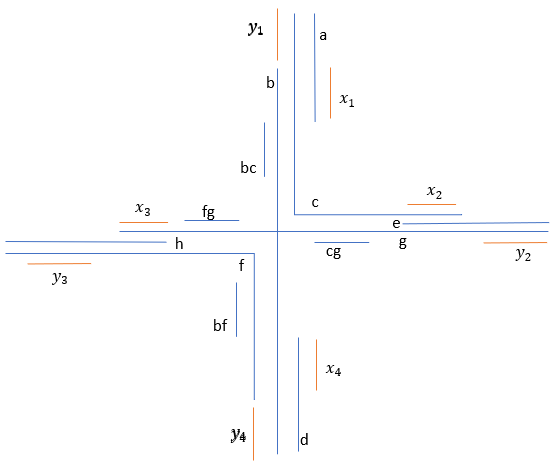
\includegraphics[width=\linewidth]{./img/representacaoFalsePieGadgetClausula.png}
%               \caption{Representação de Torta Falsa}
%               \label{fig:falsePie}
%           \end{figure}
%       \end{minipage}
%       %\hspace{0.09\linewidth}
      
%       \begin{minipage}{0.5\linewidth}
%           \begin{figure}[H]
%               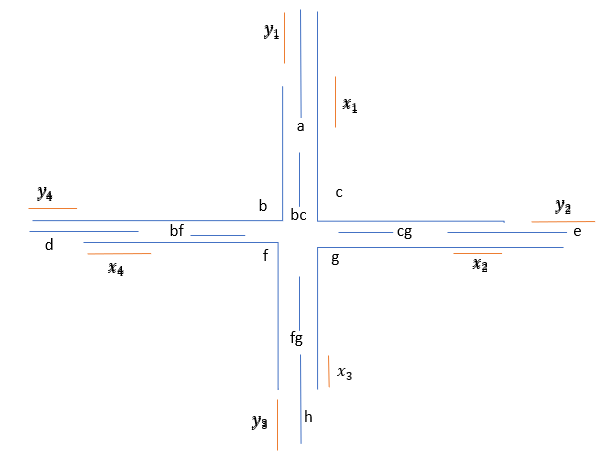
\includegraphics[width=\linewidth]{./img/representacaoTruePieGadgetClausula.png}
%               \caption{Representação de Torta Verdadeira}
%               \label{fig:truePie}
%           \end{figure}
%       \end{minipage}
 
%  \end{minipage}
      
%        \hspace{0.34\linewidth}
%       \begin{minipage}{0.5\linewidth}
%           \begin{figure}[H]
%               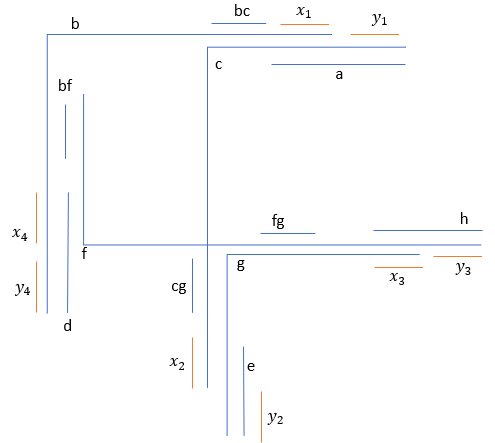
\includegraphics[width=\linewidth]{./img/representacaoFrameGadgetClausula.png}
%               \caption{Representação de Frame}
%               \label{fig:frame}
%           \end{figure}
%       \end{minipage}
      
\begin{figure}[h]
\centering
\subfloat [Representação de Torta Falsa]{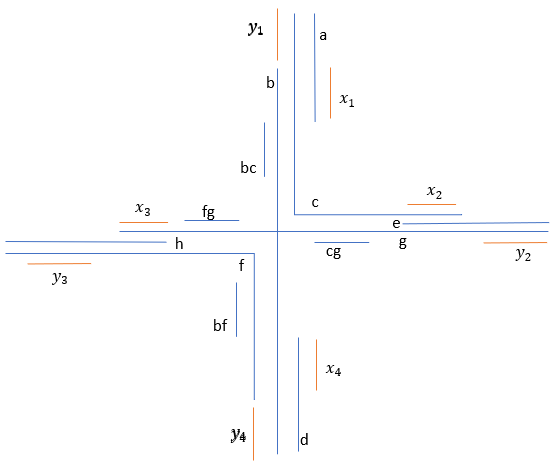
\includegraphics[width=13cm]{./img/representacaoFalsePieGadgetClausula.png}\label{fig:falsePie}}
\qquad
\subfloat[Representação de Torta Verdadeira]{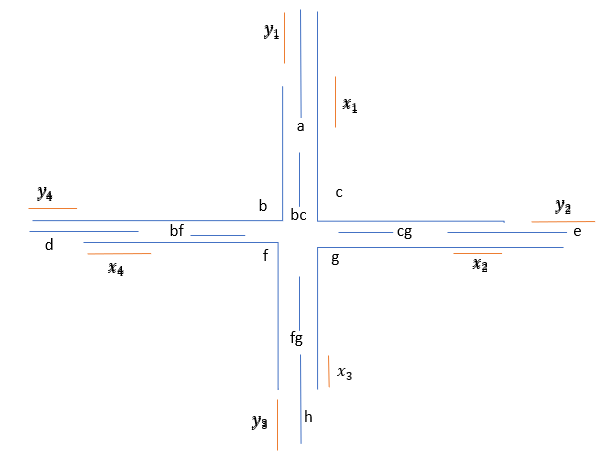
\includegraphics[width=13cm]{./img/representacaoTruePieGadgetClausula.png}\label{fig:truePie}}
\qquad
%\subfloat[][Representação de Torta Frame]{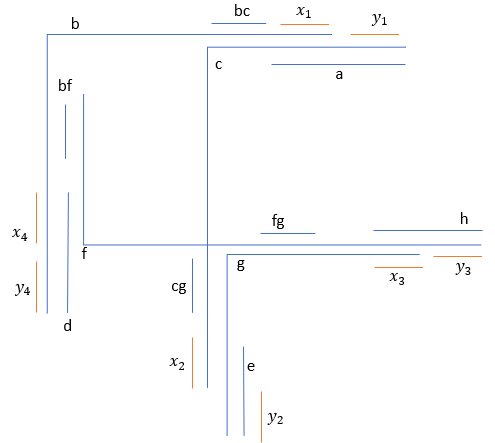
\includegraphics[width=12cm]{./img/representacaoFrameGadgetClausula.png}\label{fig:frame}}
\caption{Representações estruturais $B_{1H}(G_{C})$, como tortas. }
\end{figure}  
  
  
  
  
  
